In this chapter we will illustrate most of action allowed in CLup and CLup Operator using UI flowchart digrams. UI flowchart diagrams are used to model the interactions that users have with the software, by understanding how the system is expected to work. \\
Diagrams are built using the mockups already put in the RASD, but in a more detailed way.

\section{Mobile Interface: CLup}

\begin{figure}[H]
  \label{login_rec}
  \centering
  \makebox[\linewidth]{
  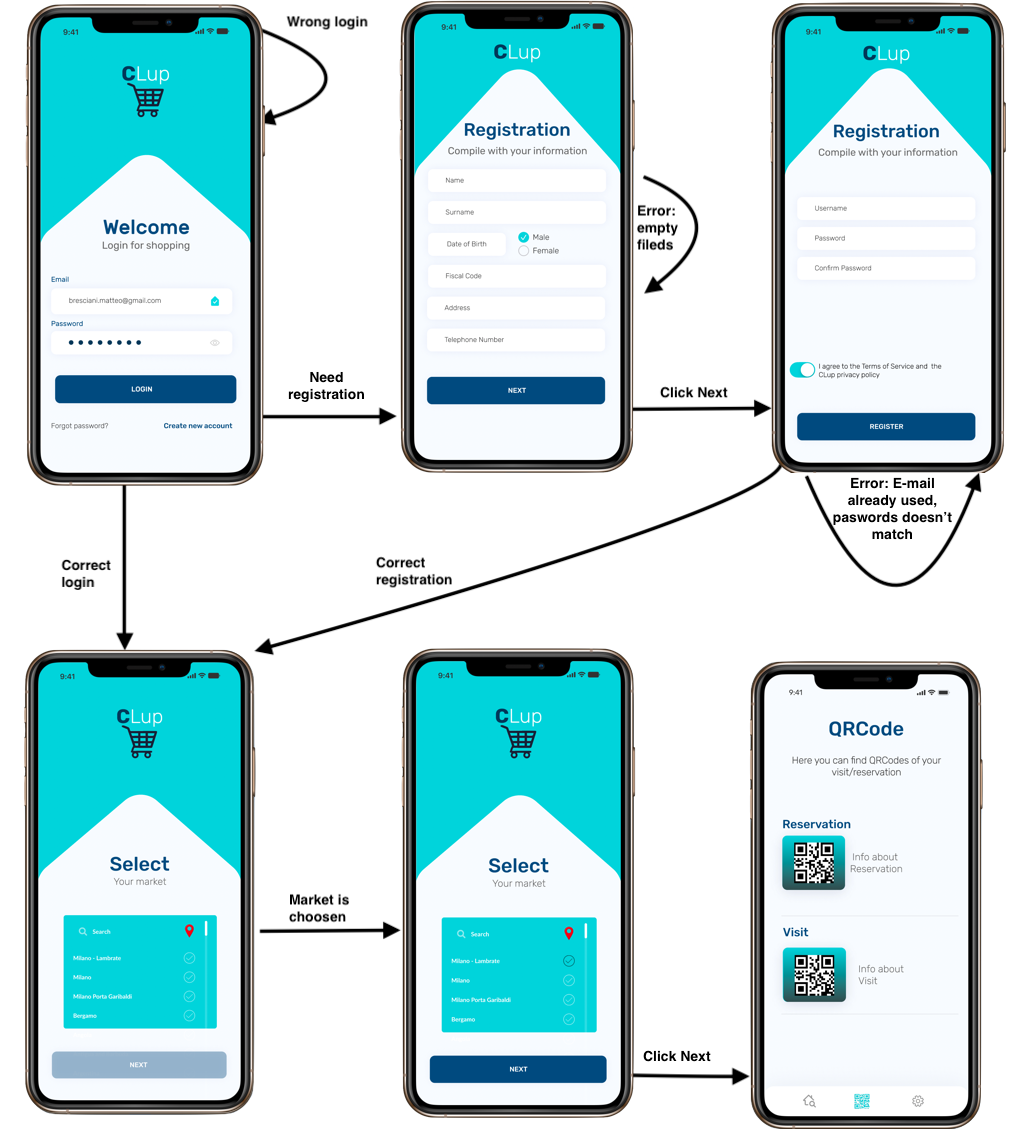
\includegraphics[scale=0.38]{images/userinterfaces/login_reg.png}}
    \caption{Login and registration interface: starting from the first screenshot the user must authenticate or register himself to use CLup. Hypothetically if a User signs up for the first access, he will be already logged in. After procedure the home screen will be displayed.}
\end{figure}



\begin{figure}[H]
  \label{menu}
   \caption{From the home screen it's possibile to move in the other three app section by selecting them in the Bottom Navigation Bar}
  \centering
  \makebox[\linewidth]{
  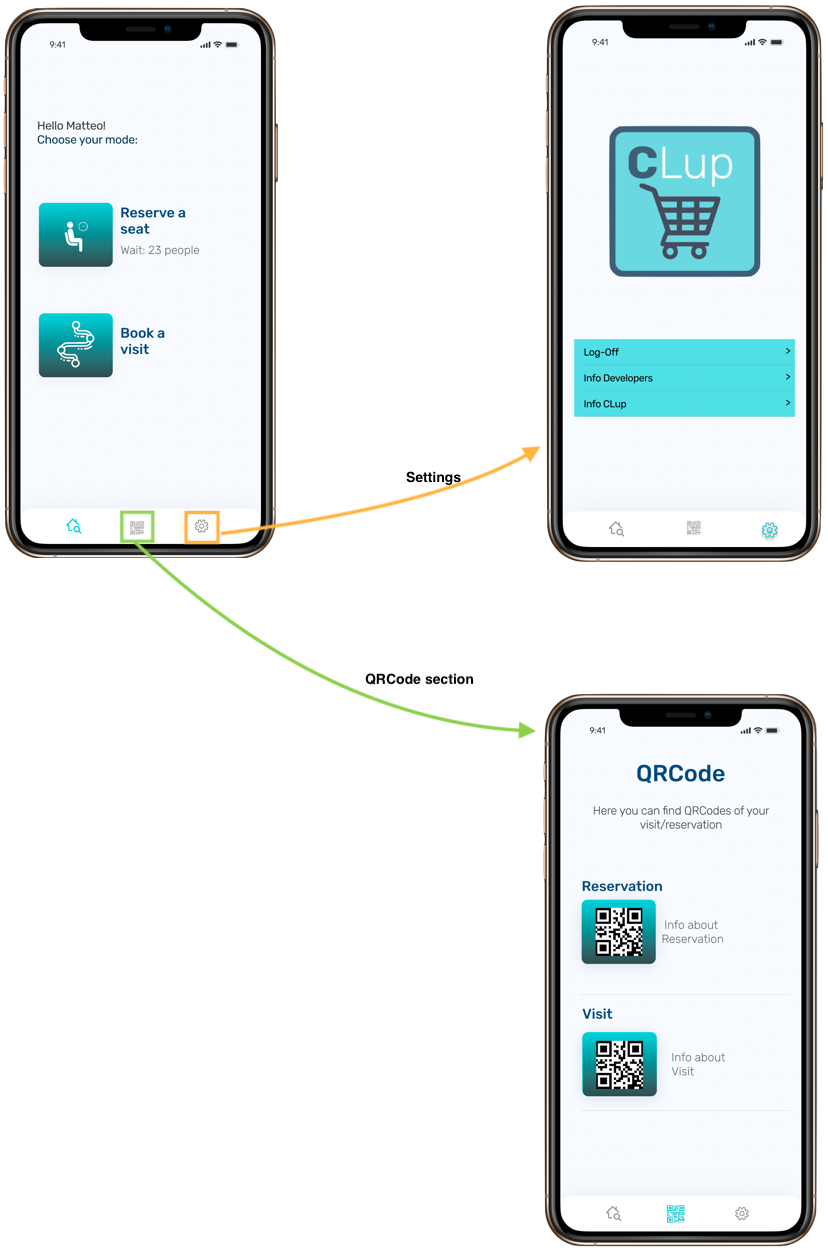
\includegraphics[scale=0.45]{images/userinterfaces/menu.png}}
   
\end{figure}



\begin{figure}[H]
  \label{Visit_steps}
  \caption{Procedure needed to book a Visit.}
  \centering
  \makebox[\linewidth]{
  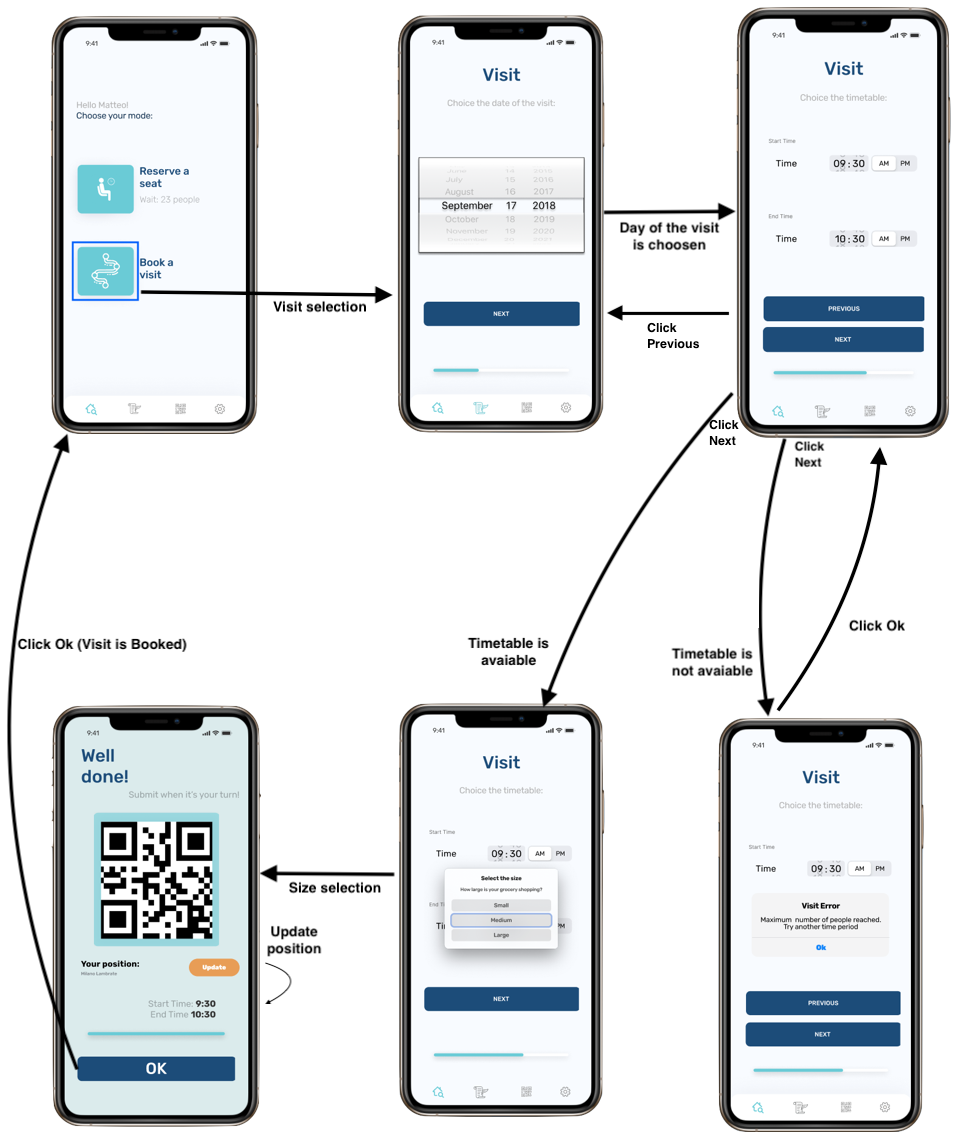
\includegraphics[scale=0.49]{images/userinterfaces/Visit_steps.png}}
\end{figure}


\begin{figure}[H]
  \label{Reservation_steps}
 \caption{Procedure needed to make a Reservation.}
  \centering
  \makebox[\linewidth]{
  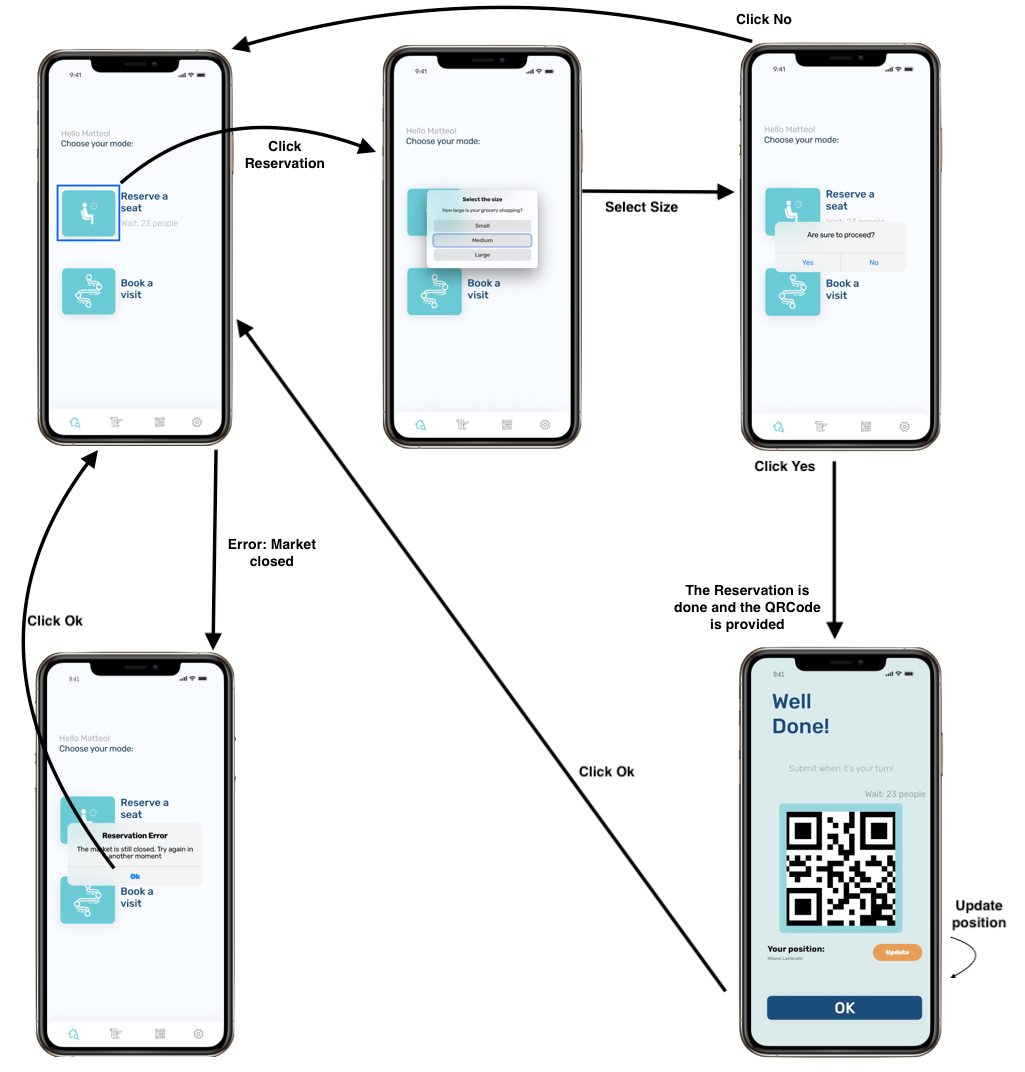
\includegraphics[scale=0.49]{images/userinterfaces/Reservation_steps.png}}
\end{figure}


\begin{figure}[H]
  \label{QRCode_handle2}
   \caption{The diagrams shows how it's possibile, from the QRCode section, to cancel a Visit. The procedure will be the same also for a Reservaiton cancellation. In particular the following screenshoots illustrate the procedure in a scenario in which a user has booked both Reservation and Visit.}
  \centering
  \makebox[\linewidth]{
  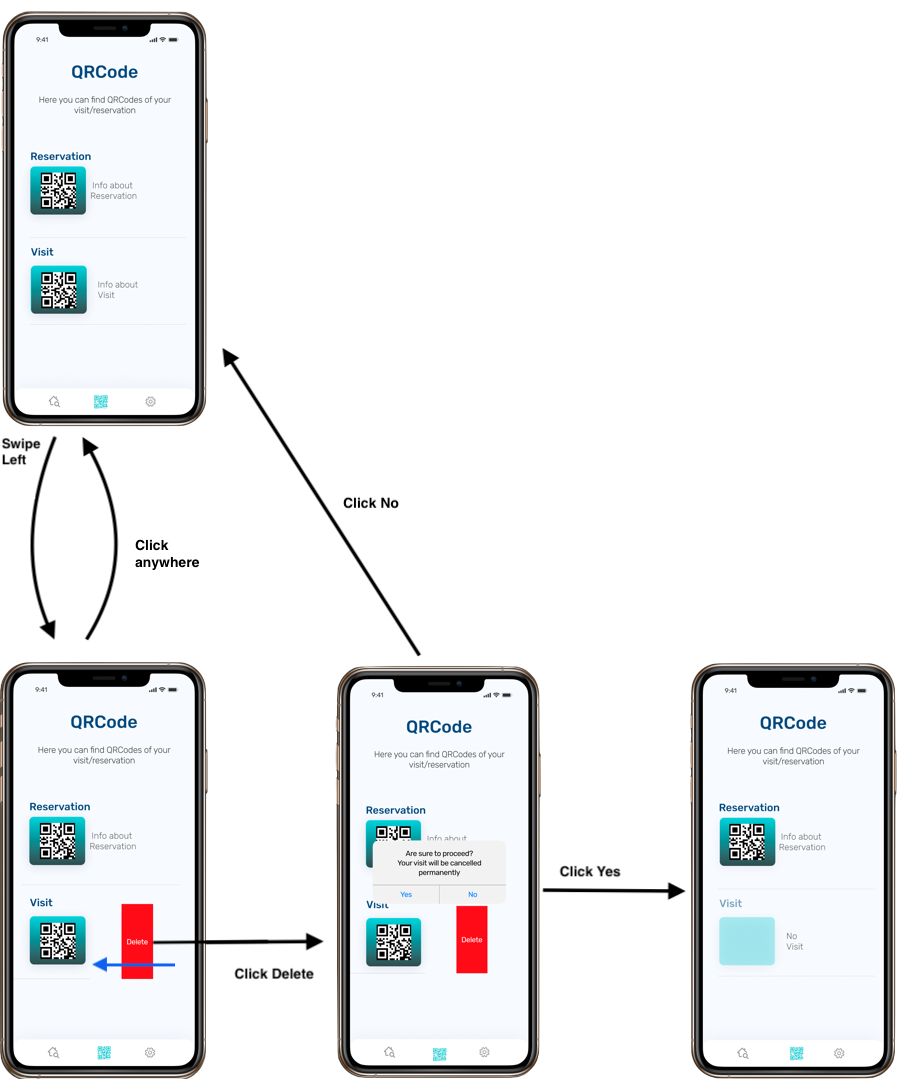
\includegraphics[scale=0.475]{images/userinterfaces/QRCode_handle2.png}}
   
\end{figure}


\begin{figure}[H]
  \label{QRCode_handle}
  \centering
   \makebox[\linewidth]{
  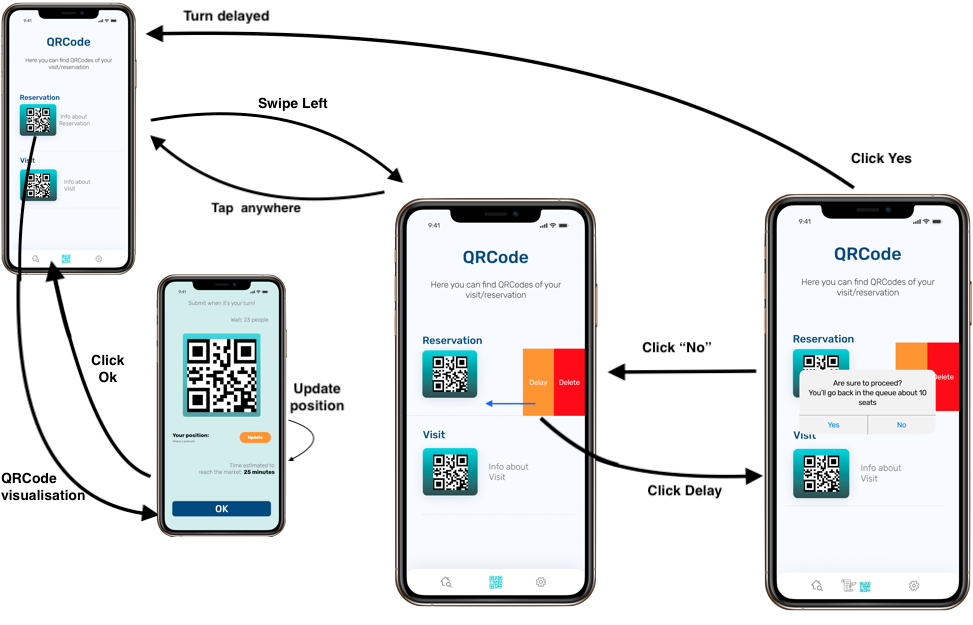
\includegraphics[scale=0.50]{images/userinterfaces/QRCode_handle.png}}
    \caption{The diagrams shows how it's possibile, from the QRCode section, to postpone the own turn in queue for a Reservation. In particular the following screenshoots illustrate the procedure in a scenario in which a user has booked both Reservation and Visit.}
\end{figure}

\section{Desktop Interface: CLup Operator}


\begin{figure}[H]
  \label{Receptionist1}
  \centering
  \makebox[\linewidth]{
  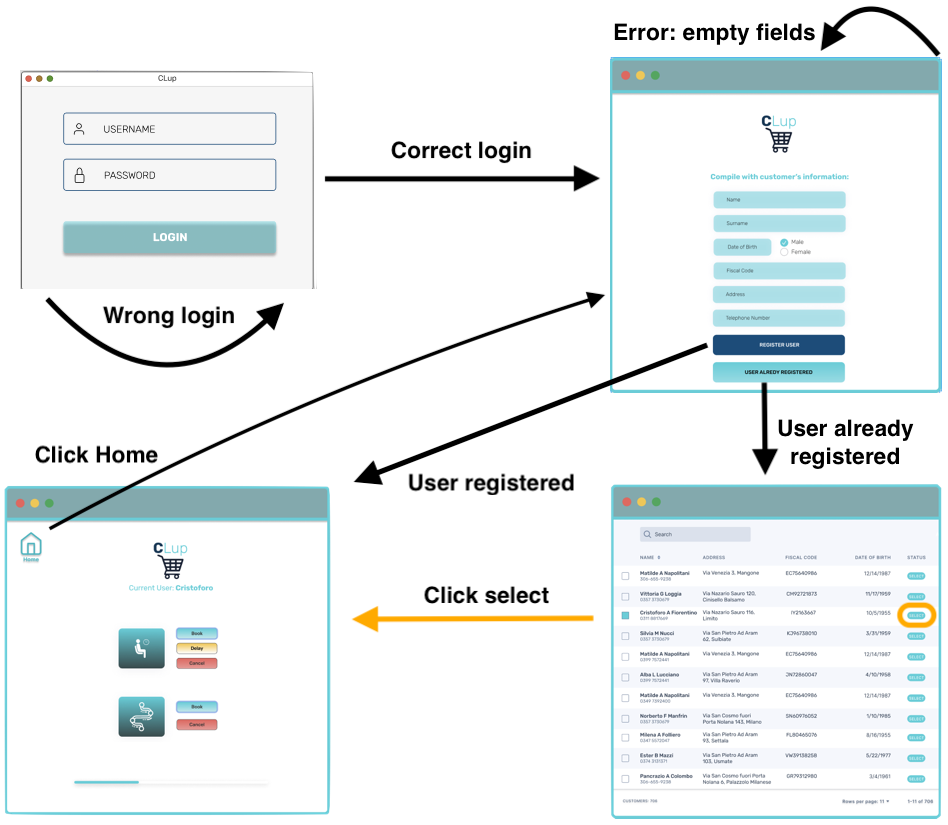
\includegraphics[scale=0.52]{images/userinterfaces/Receptionist1.png}}
    \caption{A receptionist must authenticate himself before taking into account the user's request. After this the receptionist is able to select an existing or register a new user in order to satisfy his request.}
\end{figure}


\begin{figure}[H]
  \label{Receptionist2}
  \centering
  \makebox[\linewidth]{
  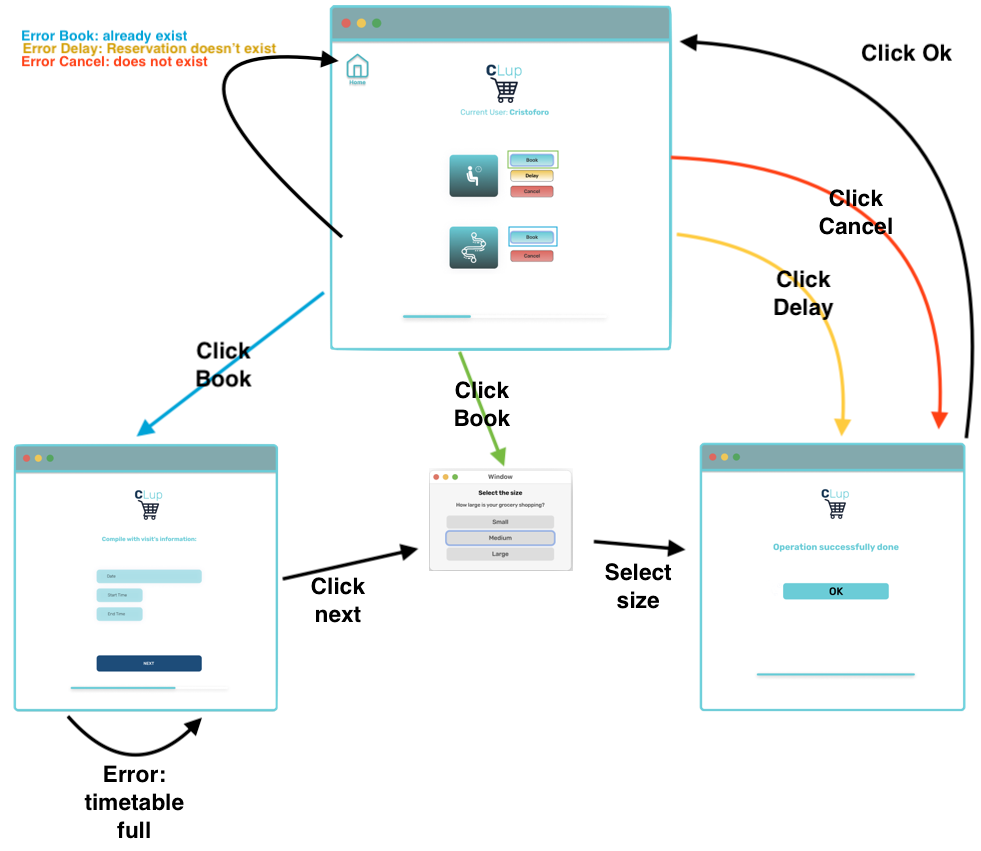
\includegraphics[scale=0.52]{images/userinterfaces/Receptionist2.png}}
    \caption{The following screenshots illustrate how a receptionist can manage user's request through some steps.}
\end{figure}

